\documentclass{beamer}

\usepackage[czech]{babel}
\usepackage[utf8]{inputenc}
\usepackage{multicol}
\usepackage[backend=biber, style=iso-numeric, alldates=iso]{biblatex}

\usetheme{Madrid}
\usecolortheme{default}% - nic / default == modrá

\title{Webová služba pro sběr a vizualizaci předpovědí počasí}
\subtitle{Web Service for Collection and Visualization of Weather Forecasts}
\author{Jan Jedlička JED0050}
\institute{VŠB-TUO}
\date{2021}

\begin{document}
	
	\frame{\titlepage}
	
	\begin{frame}
		\frametitle{Úvod}
		
		\begin{itemize}
			\item Aplikace agregující data z různých datových zdrojů
			\item Webová služba poskytující agregovaná data
			\item Aplikace zobrazující data z webové služby
		\end{itemize}
		
	\end{frame}

	\begin{frame}
		\frametitle{Řešení}
		
		\begin{itemize}
			\item Knihovny jednotlivých datových zdrojů
			\item Knihovna pro správu různých datových zdrojů
			\item ASP.NET aplikace využívající knihovnu agregace dat
			\item WinForm aplikace zobrazující data z webu
		\end{itemize}
		
		\begin{figure}
			
			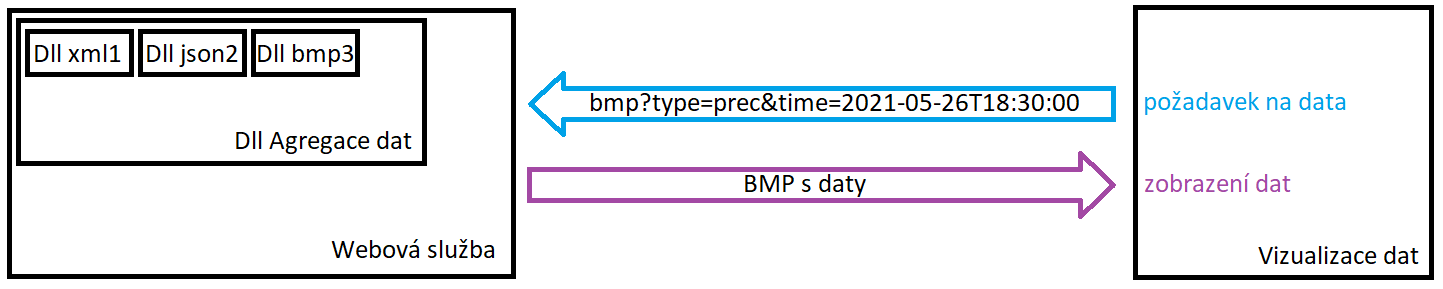
\includegraphics[scale=0.323]{figures/schema prace.png}

		\end{figure}
		
	\end{frame}

	\begin{frame}
		\frametitle{Datové zdroje}
		
		\begin{itemize}
			\item XML
			\begin{itemize}
				\item Yr.no
			\end{itemize}
			\item JSON
			\begin{itemize}
				\item OpenWeather
				\item WeatherUnlocked
			\end{itemize}
			\item BMP
			\begin{itemize}
				\item Medard
				\item Radar.bourky
			\end{itemize}
		\end{itemize}
	\end{frame}

	\begin{frame}
		\frametitle{Porovnání datových zdrojů}
		
		\begin{tabular} {l r c c c c c c c}
			
			Zkratka & Typ & Dny & Hodin rozdíl & Stažení/min & Plocha & Prvek \\
			\hline
			Yrno & XML & 9 & 1 a 6 & & svět & s,v,t1,t2 \\ 
			Owm & JSON & 5 & 3 & 60 & svět & s,v,t1,t2 \\ 
			Weun & JSON & 5 & 3 & 75 & svět & s,v,t1,t2 \\ 
			Mdrd & BMP & 5 & 1 &  & Evropa & s,t1 \\ 
			Rb & BMP & -3 & 0.16 (10 min)& & ČR & s \\ 
			\multicolumn{7}{r}{\footnotesize *s = srážky, v = vlhkost, t1 = teplota, t2 = tlak}\\
		\end{tabular}
	\end{frame}
	
	\begin{frame}
		\frametitle{Agregace dat}
		
		\begin{itemize}
			\item Škála
			\item Triangulace
			\item Interpolace
			\item Data
		\end{itemize}
	\end{frame}

	\begin{frame}
		\frametitle{Distribuce dat}
		
		\begin{itemize}
			\item Bitmap předpověď
			\item XML a JSON předpověď
			\item Ohraničení bitmapy
			\item Využité škály
		\end{itemize}
		
	\end{frame}

	\begin{frame}
		\frametitle{Vizualizace dat}
		
		\begin{itemize}
			\item Počasí v bodě
			\item Počasí na trase
			\item Animace předpovědi
		\end{itemize}
	
	\end{frame}

	\begin{frame}
		\frametitle{Zhodnocení}
		
		\begin{itemize}
			\item Jednoduchá práce s daty
			\item Dynamické rozšíření o nové datové zdroje
			\item Splnění všech požadavků
			\item Pomalé zpracovávání více datových zdrojů současně
			\item Nedostatečně promyšlený návrh
		\end{itemize}
	\end{frame}

	\begin{frame}
		\frametitle{Poděkování}
		
		\begin{center}
			\Huge
			Děkuji za pozornost
		\end{center}
		
	\end{frame}
	
\end{document}